% ==============
% PARAMETRAGES
% à compiler en pdfLaTeX
% ==============

% GENERAL
%  type de document rapport, chapitre commence en page impaire ou paire indifféremment
\documentclass[twoside,a4paper,11pt,frenchb,openany]{report}  
%  type de document, chapitre commence en page impaire
%\documentclass[twoside,a4paper,12pt,frenchb,openright]{report} 
\title{Etat de l'art du projet de recherche}
\author{Stephane Robin}
\date{\today}

% IMPORTATION DE LIBRAIRIES
\usepackage{amssymb}  % symboles
\usepackage{amsmath}  % symboles mathématiques
\usepackage{amsfonts}  % polices de caractères
\usepackage{amscd}
\usepackage{amsthm}  % symboles mathématiques pour redéfinir les théorèmes
\usepackage[all,cmtip]{xy}
\usepackage{array}  % tableaux
\usepackage[frenchb]{babel}  % langue française
\usepackage{bm}  % caractères grecs
\usepackage{calc}
\usepackage[justification=centering]{caption} % centralise les légendes des figures
\usepackage{enumitem} % listes
\usepackage{eurosym}  % symbole euro
\usepackage{euscript}
\usepackage{fancybox}  % boîtes
\usepackage{float}  % images flottantes
\usepackage[T1]{fontenc}  % LaTeX modele
\usepackage[top=3.1cm,bottom=2.7cm,left=2.2cm,right=2.2cm,dvips]{geometry}  % marges
\usepackage{graphicx}  % insertion images
\usepackage[utf8]{inputenc}  % accents
\usepackage{mathrsfs}  % symboles mathématiques
\usepackage{mathtools}  % outils mathématiques
\usepackage{mdframed} % box autour des theoremes
\usepackage{pst-plot, pstricks}
\usepackage{pstricks-add}
\usepackage{rotating}
\usepackage{setspace} % permet de définir l'espace entre les lignes
\usepackage{srcltx}
\usepackage{textcomp}   % caracteres complementaires
\usepackage{titlesec}  % sections
\usepackage{titletoc}  % table de contents
%\usepackage[nottoc,notlof,notlot]{tocbibind}  % bibliothèque
\usepackage{verbatim}  % caracteres non interpretes
\usepackage{wrapfig}  % pour inserer les figures dans du texte

% COULEURS
\definecolor{couleurTitre}{RGB}{64,128,128}  % doit être défini avant xcolor
\definecolor{couleurUrl}{RGB}{127,62,0}
\usepackage{xcolor}  % couleurs
%\definecolor{amber}{rgb}{1.0,0.49,0.0} % couleur non utilisee
%\definecolor{greyish}{rgb}{52.0,160.0,157.0} % couleur non utilisee
%\definecolor{theoremeCouleur}{rgb}{224.0,90.0,67.0} % couleur non utilisee
	
% LISTES
\renewcommand{\labelitemi}{$\bullet$}  % symboles de listes
\frenchbsetup{StandardLists=true}  % style de bullets

% IMAGES
\usepackage{caption}  % insertion d'images
\usepackage[font=footnotesize,labelfont=bf]{caption}  % légendes des images
\renewcommand{\thefigure}{\arabic{section}.\arabic{figure}}  % numérotation des images
\usepackage{subcaption}

% HYPERLINKS
\usepackage{hyperref}
\hypersetup{
colorlinks=true,
linkcolor=couleurUrl,
citecolor=couleurUrl,
urlcolor=couleurUrl,
breaklinks=true % saute la ligne au milieu d'un href
}
\PassOptionsToPackage{hyphens}{url}\usepackage{hyperref} % pour que url ait les memes propriétés que hyperref

% LIGNES
\usepackage{parskip}
%\setlength\parskip{\baselineskip} % joint a la suppression de l'espace horizontal
%\setlength{\parindent}{0cm} % supprime l'espace horizontal en debut de ligne

% HEADINGS AND FOOTERS
\usepackage{fancyhdr}  % entete
\pagestyle{fancy}  % la page accepte les entetes et pieds de page
\renewcommand{\headrulewidth}{0pt}
\fancyhead[L,R,C]{}
%\fancyhead[LE]{} % pages paires header gauche
%\fancyhead[CE]{} % pages paires header centre
%\fancyhead[RE]{Le théorème de Pythagore} % pages paires header droit
%\fancyhead[LO]{Le théorème de Pythagore} % pages impaires header gauche
%\fancyhead[CO]{} % pages impaires header centre
%\fancyhead[RO]{} % pages impaires header droit
%\fancyfoot[c]{\textcolor{gray}{\thepage}}  % pied de page
%\fancyfoot[L,R,C]{} % forcing footer empty

% REDEFINITION DU STYLE DE THEOREM
\newmdtheoremenv[  % definitions
linewidth=5,
leftline=true,
rightline=false,
bottomline=false,
topline=false,
leftmargin=0,
rightmargin=0,
backgroundcolor=couleurTitre!20,
linecolor=orange!70,
innertopmargin=21pt,
skipabove=\topskip,
ntheorem=true]{definition}{Définition}

\newmdtheoremenv[  % theoremes
linewidth=5,
leftline=true,
rightline=false,
bottomline=false,
topline=false,
leftmargin=0,
rightmargin=0,
backgroundcolor=couleurTitre!20,
linecolor=orange!70,
innertopmargin=10pt,
skipabove=\topskip,
ntheorem=true]{theorem}{}

\newmdtheoremenv[  % proprietes
linewidth=5,
leftline=true,
rightline=false,
bottomline=false,
topline=false,
leftmargin=0,
rightmargin=0,
backgroundcolor=couleurTitre!20,
linecolor=orange!70,
innertopmargin=21pt,
skipabove=\topskip,
ntheorem=true]{property}{Propriété}

\newmdtheoremenv[  % propositions
linewidth=5,
leftline=true,
rightline=false,
bottomline=false,
topline=false,
leftmargin=0,
rightmargin=0,
backgroundcolor=couleurTitre!20,
linecolor=couleurTitre!70,
innertopmargin=21pt,
skipabove=\topskip,
ntheorem=true]{proposition}{Proposition}

\newmdtheoremenv[  % corollaires
linewidth=5,
leftline=true,
rightline=false,
bottomline=false,
topline=false,
leftmargin=0,
rightmargin=0,
backgroundcolor=couleurTitre!20,
linecolor=couleurTitre!70,
innertopmargin=21pt,
skipabove=\topskip,
ntheorem=true]{corollary}{Corollaire}

\newmdtheoremenv[  % lemmes
linewidth=5,
leftline=true,
rightline=false,
bottomline=false,
topline=false,
leftmargin=0,
rightmargin=0,
backgroundcolor=couleurTitre!20,
linecolor=couleurTitre!70,
innertopmargin=21pt,
skipabove=\topskip,
ntheorem=true]{lemma}{Lemme}

% NUMEROTATION DES CHAPITRES-SECTIONS
\renewcommand{\theequation}{\arabic{chapter}.\arabic{equation}}  % equations
%\renewcommand{\theequation}{\thesection\arabic{equation}}  % equations
%\numberwithin{equation}{section}  % equations

%\renewcommand{\thepart}{\Alph{part}}  % parties
%\renewcommand{\thechapter}{\arabic{chapter}.}  % chapitres
\renewcommand{\thesection}{\arabic{section}.}  % sections
\renewcommand{\thesubsection}{\arabic{section}.\arabic{subsection}.}  %  sous-sections
\renewcommand{\thesubsubsection}{\arabic{section}.\arabic{subsection}.\arabic{subsubsection}.}  % sous-sous-sections

\renewcommand{\thedefinition}{\arabic{chapter}.\arabic{definition}}  % definitions
\renewcommand{\theorem}{}  % theoremes
\renewcommand{\theproperty}{\arabic{chapter}.\arabic{property}}  % property
\renewcommand{\theproposition}{\arabic{chapter}.\arabic{proposition}}  % propositions
\renewcommand{\thecorollary}{\arabic{chapter}.\arabic{corollary}}  % corollaires
\renewcommand{\thelemma}{\arabic{chapter}.\arabic{lemma}}  % lemmes
\setcounter{secnumdepth}{4}  % profondeur de numérotation

% FORMAT DES SECTIONS-TITRES
\titleformat{\section}{\normalfont\normalsize\bfseries}{\textcolor{couleurTitre}{\thesection}}{1.2em}
{\normalfont\large\bfseries\scshape\textcolor{couleurTitre}} % format de titre de section
\titleformat{\subsection}{\normalfont\normalsize\bfseries}{\textcolor{couleurTitre}{\thesubsection}}{1em}
{\normalfont\normalsize\bfseries\textcolor{couleurTitre}}  % format de titre de sous-section
\titleformat{\subsubsection}{\normalfont\normalsize\bfseries\itshape}{\textcolor{couleurTitre}{\thesubsubsection}}{1em}
{\normalfont\normalsize\bfseries\itshape\textcolor{couleurTitre}}  % format de titre de sous-sous-section

\makeatletter

% CONCERNE LA TABLE DES MATIERES
%\renewcommand{\@chapapp}{}  % le mot `chapitre'' n'apparait plus en titre de chapitre
\renewcommand\l@section{\@dottedtocline{1}{0em}{1.5em}}  % espacement dans le titre d'une section
\renewcommand\l@subsection{\@dottedtocline{1}{2.5em}{2.5em}}  % espacement dans le titre d'une sous-section
\renewcommand\l@subsubsection{\@dottedtocline{1}{5em}{2.5em}}  % espacement dans le titre d'une sous-sous-section

\makeatother

% ==============
% DEBUT DU DOCUMENT
% ==============

\begin{document}

\maketitle

\tableofcontents

\section{Introduction}

Le présent document cherche à définir les fondements sur lesquels va reposer le stage et en particulier de connaître l'état actuel des connaissances concernant l'analyse bioinformatique du locus CRISPR-Cas chez \textit{Mycobacterium tuberculosis}.

L'objectif du stage est de comprendre les liens entre les sept lignées de \textit{M. tuberculosis} et les alternances de gènes et espaceurs du locus CRISPR-Cas, au moyen d'outils développés au sein de l'équipe AND de l'Université de Franche Comté.


% OUT OF AFRICA MIGRATION ========================================================

\section{Evolution de la branche humaine de la tuberculose}

% Diversité génétique de la tuberculose

\subsection{Diversité génétique de la tuberculose}

Le polymorphisme génétique est à l'origine de la diversité génétique et correspond à des variations de séquences d'ADN entre différentes souches de \textit{M. tuberculosis}. Ces variations sont dues à des mutations successives au cours de l'évolution de la bactérie, et elles permettent l'analyse phylogénique de \textit{M. tuberculosis}. Il existe plusieurs formes de polymorphisme, le polymorphisme chromosomique lié à un changement du nombre de chromosomes ou de leurs structures, le polymorphisme d'insertion, de délétion et d'inversion qui provoquent un changement spécifique de certaines séquences du génome, et le polymorphisme nucléotidique SNP \textit{Single Nucleotide Polymorphism} lié au changement d'une seule paire de bases\footnote{\textbf{Paire de bases} : appariement de 2 bases nucléiques situées sur 2 brins complémentaires d'ADN, reliées par des ponts d'hydrogène.} du génome de \textit{M. tuberculosis}. Ce dernier cas est au coeur de notre étude.

Certaines mutations n'ont aucun impact évolutif sur \textit{M. tuberculosis}. En revanche, des changements fonctionnels peuvent avoir lieu lorsque ces mutations entraînent des modifications d'acides aminés dans les régions codantes, cela peut-être le cas lors d'une adaptation à l'environnement ou lors d'une nouvelle forme de résistance aux antibiotiques. Les SNPs synonymes ne changent pas la séquence de protéine, ainsi la substitution d'un codon\footnote{\textbf{Codon} : ensemble composé de trois nucléotides consécutifs spécifiant l'incorporation d'un acide aminé déterminé. Le code génétique est ainsi lu trois nucléotides par trois nucléotides.} par un autre codon peut engendrer le même acide aminé. Au contraire, les SNPs non-synonymes changent la séquence de protéine, et engendrent donc l'incorporation d'un acide aminé différent. Les SNPs sont peu sujets à des phénomènes d'homoplasie\footnote{\textbf{Homoplasie} : similitude de caractères chez différentes espèces, qui ne provient pas d'un ancêtre commun, mais peut par exemple provenir d'une adaptation à l'environnement. Diffère de l'homologie qui est une similitude de caractères observée chez deux espères différentes, provenant de l'héritage d'un ancêtre commun.}(seuls 1,1 \% des SNPs sont homoplasiques), ce qui suggère que la structure de \textit{M. tuberculosis} favorise les clonages plutôt que les recombinaisons entre branches. Pour de tels organismes clonaux, l'identification de mutations homoplasiques est un excellent moyen de déterminer les différentes souches bactériennes, et de procéder à des études phylogéniques\footnote{\textbf{Phylogénie} : étude des liens entre espèces apparentées, permettant de retracer les principales étapes de l'évolution des organismes depuis un ancêtre commun.} et de classification.

% Co-évolution de la tuberculose avec l'homme moderne

\subsection{Co-évolution de la tuberculose avec l'homme moderne}

Le développement des maladies s'adapte à la densité de population concernée. En effet, auprès d'une foule dense, les infections se répandent plus largement et deviennent plus virulentes, alors qu'auprès d'une population moins importante, elles ont une croissance plus faible, laissant parfois place à des périodes où les infections restent latentes.

Une période charnière dans l'histoire de l'humanité est la transition démographique du Néolithique, qui a vu il y a 10 000 ans, suite à l'apparition de l'agriculture et de l'élevage, un accroissement de la population, favorisant la naissance de nombreuses maladies. Les maladies humaines plus anciennes se développaient auprès de populations moins denses et produisaient des phases chroniques de latence et de réactivation permettant aux populations infectées de survivre.

La tuberculose conjugue ces deux modèles de maladie. En effet, elle a montré à travers les âges des périodes de réactivation, elle dépend par ailleurs fortement de la densité de population et son mode de transmission aérosol s'est parfaitement adapté aux foules.

% The global diversity of human-adapted MTBC

L'étude phylogénique de Comas et al.\cite{comas} se base exclusivement sur l'étude du génome\footnote{\textbf{Génome} : ensemble de l'information génétique d'un organisme. Par extension, le génome se réfère aussi au support physique de cette information génétique, la macromolécule d'ADN. L'annotation des gènes est le processus permettant d'identifier l'emplacement des gènes dans l'ADN, de déterminer leurs fonctions et leurs possibles interactions.} complet de toutes les lignées connues de \textit{M. tuberculosis} en utilisant les SNPs comme marqueurs pour construire les relations entre les différentes branches. Les résultats obtenus rejoignent de précédentes études effectuées à partir d'autres marqueurs, et confirment l'existence de sept principales lignées de tuberculose. On remarque en particulier que plusieurs branches d'origine animale se sont regroupées avec la lignée 6 d'Afrique de L'Ouest, et que les lignées modernes 2 d'Asie de l'Est, 3 d'Asie Centrale et 4 d'Europe ont des origines proches. 

% African origin and co-divergence of MTBC with modern humans

L'analyse phylogénique de Comas et al. corrobore la conjecture selon laquelle la tuberculose est originaire d'Afrique. Par ailleurs, s'appuyant sur les origines africaines de l'espèce humaine, cette étude cherche également à déterminer l'ancienneté de l'association entre la tuberculose et son hôte humain. L'analyse des divergences des génomes de la tuberculose est comparée à celle d'une arborescence génétique déjà établie à partir de mitochondries\footnote{\textbf{Mitochondrie} : centrale énergétique des cellules qui contribue à la production d'ATP.} de l'être humain. 

% Age of the association of MTBC and humans

Les similitudes relevées montrent que la tuberculose a infecté les premiers hommes d'Afrique. Pour aller plus loin, l'étude de Comas et al. a tenu compte de trois dates importantes dans l'évolution de l'être humain qui ont été reportées sur l'analyse phylogénique de \textit{M. tuberculosis} des lignées 5 et 6 d'Afrique de l'Ouest :

- l'émergence de l'homo sapiens correspondant au MTBC-185\footnote{\textbf{MTBC} : Mycobacterium Tuberculosis Complex.},\\
- l'émergence du haplogroupe\footnote{\textbf{Haplogroupe} : groupe possédant les mêmes caractères génétiques et partageant un ancêtre commun suivant une mutation SNP.} mitochondriaque de la lignée 3 chez l'homme correspondant au MTBC-70,\\
- le début de la transition démographique du Néolithique correspondant au MTBC-10.

La branche MTBC-70 a révélé des corrélations avec l'histoire de l'humanité telle qu'elle a été décrite par l'archéologie, en montrant l'apparition des sept différentes lignées de tuberculose :

- il y a 73 000 ans, apparition des lignées 5 et 6 correspondant à une 1ère migration humaine importante vers l'Afrique de l'Ouest,\\
- il y a 67 000 ans, apparition de la lignée 1 correspondant à une migration humaine importante autour de l'Océan Indien,\\
- il y a 64 000 ans, apparition de la lignée 7 concernant une population qui est restée en Afrique ou est revenue en Afrique après une première migration,\\
- il y a 46 000 ans, apparition de la lignée 4 correspondant à une migration humaine importante vers l'Europe,\\
- il y a 42 000 ans, apparition des lignées 2 et 3 correspondant à une migration humaine importante vers l'Asie de l'Est et l'Asie Centrale. 

\begin{figure}[h!]
\centering
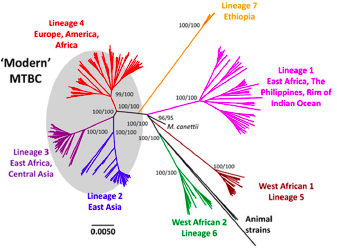
\includegraphics[scale=0.7]{worldlignee.png}
\caption{Philogénie du génome complet de MTBC, d'après\\ \textit{Out-of-Africa migration and Neolithic coexpansion of Mycobacterium\\tuberculosis with modern humans}}
\end{figure}

En revanche, la branche MTBC-185 suggère l'apparition de mutations à partir de lignées africaines il y a 174 000 ans, c'est à dire que la dispersion de la tuberculose précèderait celle de l'homo sapiens.

% Neolithic co-expansion of MTBC and humans

Dans tous les cas, la tuberculose aurait infecté l'espèce humaine et évolué conjointement avec elle depuis 70 000 ans, mais son apparition serait antérieure à la transition démographique du Néolithique.

La base de données de tuberculose étudiée de façon probabiliste par Comas et al.\cite{comas} montre que le Néolithique a fortement contribué à l'expansion de la maladie il y a 10 000 ans grâce à l'augmentation de la densité de population, à la probabilité de co-infection avec d'autres maladies également dépendantes de la densité de population, et non pas grâce à la possibilité pour la tuberculose de muter d'une variété animale vers une variété humaine. En effet, l'analyse phylogénique de la tuberculose montre que les branches humaines ont divergé des branches animales avant le Néolithique.

Le Néolithique n'était pas la seule période où l'augmentation de la population fut importante, toutefois la concentration de population qui s'en est suivie a permis l'apparition auprès de la tuberculose de caractères fortement dépendants de la densité de population qu'elle affecte. Le Néolithique a donc marqué un tournant dans l'histoire de la tuberculose qui a alors commencé à conjuguer les deux modèles de maladie, dépendant à la fois de la densité de population et chronique par périodes de réactivation.

% The evolutionary history of MTBC at a regional scale
% Conclusion

Il faut donc considérer que la co-existence de la tuberculose avec l'espèce humaine depuis des milliers d'années a conduit la maladie à s'adapter aux changements du génome humain et inversement. Les prochaines études sur la tuberculose devraient donc se concentrer sur des génomes complets de la tuberculose et de l'être humain choisis en rapport à leurs associations.

En particulier, la tuberculose a dû s'adapter aux autres infections ayant touché l'espèce humaine, avec plus ou moins de succès. Dans cet ordre d'idée, une étude récente de Perry S. et al.\cite{perry1, perry2} suggère que l'infection d'un organisme par \textit{Helicobacter Pylori} pourrait protéger de la tuberculose sous sa forme active. A contrario, nous ne savons pas si la tuberculose latente pourrait protéger contre les ulcers et les cancer de l'estomac causés par \textit{Helicobacter Pylori}.

\begin{figure}
\centering
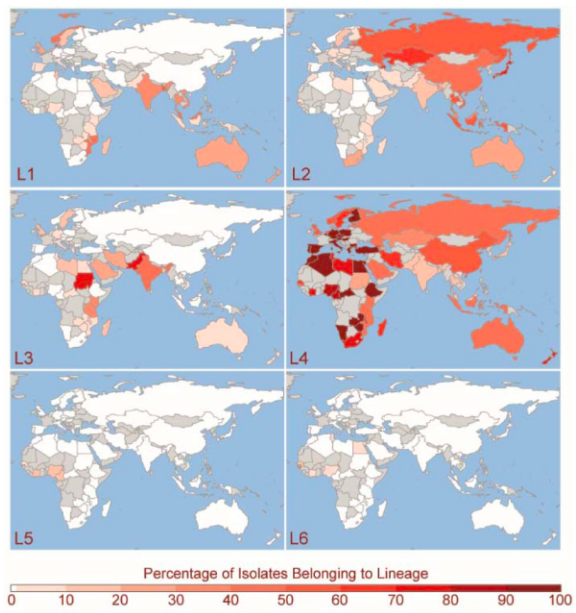
\includegraphics[scale=0.5]{world.png}
\caption{Distribution géographique des lignées 1 à 6, d'après \textit{Lineage\\ specific histories of Mycobacterium tuberculosis dispersal in Africa and Eurasia}}
\end{figure}

%  GLOBAL EXPANSION OF MTBC LINEAGE 4 =============================================

\section{Le développement de souches résistantes aux antibiotiques}

\subsection{L'expansion de la lignée 4 de \textit{M. tuberculosis}}

% global diversity of L4

La lignée 4 de \textit{M. tuberculosis} est la plus répandue de par le monde et pour cette raison a fait l'objet de nombreuses publications. Brynildsrud O.B. et al.\cite{brynildsrud} montrent que la dispersion de la lignée 4 est liée à l'expansion coloniale européenne en Afrique et en Amérique entre le 17ème et le 19ème siècle.

% phylogeographic inference

Brynildsrud O.B. et al. utilisent des méthodes d'analyse discrète et une approche bayésienne\footnote{\textbf{Approche bayésienne} : méthode probabiliste basée sur le calcul des probabilités postérieures des arbres phylogéniques par la combinaison d'une probabilité antérieure avec la fonction de vraisemblance} en phylogénie moléculaire pour obtenir de manière formelle l'évolution phylogéographique de la lignée 4 de \textit{M. tuberculosis}. Ils estiment que le plus récent ancêtre commun MRCA de la lignée 4 est apparu en Europe en 1096 après JC. Si on considère l'Europe en tant que continent dans un sens large, cela ne contredit pas les résultats de O'Neil M.B. et al.\cite{oneil} qui estiment l'origine de la lignée 4 autour de la méditerranée.

% Patterns of L4 migration through time

L'analyse phylogéographique de Brynildsrud O.B. suggère que les premières vagues de migration de la lignée 4 hors d'Europe se sont déroulées au début du 13ème siècle vers l'Asie du Sud-Est. En particulier, il est possible d'établir une correspondance entre la structure des isolats Vietnamiens et l'époque de l'expansion coloniale française en Indochine.

Les vagues suivantes de migration de la lignée 4 se sont dirigées vers l'Afrique de l'Ouest au 15ème siècle, puis vers Afrique de l'Est et du Sud au 17ème siècle. Les échanges continus avec le Portugal au 15ème siècle ont favorisé la dispersion de la maladie, ce qui a été renforcé plus tard par la colonisation française de l'Afrique de l'Ouest.  Ces échanges avec les populations européennes ont prévalu à une transmission locale de la tuberculose jusqu'au 19ème siècle. 

La première migration interne de la maladie en Afrique date de l'Empire Zulu au 19ème siècle et se dirigeait vers le Nord et l'Est africain.

La transmission de la maladie en Amérique date, quant à elle, du 15ème siècle avec la colonisation du continent, mais il faudra attendre le 17ème siècle pour voir l'explosion de la maladie en Amérique du Sud. Ce retard dans l'évolution de la maladie par rapport à la branche africaine peut s'expliquer par le taux de mortalité élevé des populations aborigènes au contact des européens.

% antibiotiques

\subsection{L'adaptation de la lignée 4 pour devenir résistante aux antibiotiques}

Nous avons déjà vu que la tuberculose a su s'adapter à l'évolution géographique de l'humanité en suivant les différentes migrations humaines pour créer de nouvelles lignées. Il apparaît que la tuberculose est également capable de suivre l'évolution médicale de l'humanité. L'étude de Brynildsrud O.B. et al. \cite{brynildsrud} constate chez \textit{M. tuberculosis} l'émergence croissante d'une résistance à de multiples antibiotiques entre 1960 et 2000 au travers de la phylogénie de la lignée 4. Des mutations spontanées dans le génome de la tuberculose peuvent altérer les protéines qui sont la cible des médicaments, ce qui rend les bactéries résistantes à ces médicaments. Prenons comme exemple une mutation du gène rpoB de \textit{M. tuberculosis}, qui code pour la sous-unité $\beta$\footnote{\textbf{Sous-unité $\beta$} : élément de l'ARN polymérase des bactéries qui est composé de la structure suivante $\alpha_2 \beta \beta' \omega$} de l'ARN polymérase\footnote{\textbf{ARN polymérase} : complexe enzymatique responsable de la synthèse de l'ARN à partir d'ADN.} de la bactérie. Dans la tuberculose non résistante, la rifampicine se lie à cette sous-unité $\beta$ et perturbe l'élongation de la transcription de l'ARN. La mutation dans le gène rpoB modifie la séquence des acides aminés et donc de la sous-unité $\beta$. Dans ce cas, la rifampicine ne peut plus se lier à l'ARN et empêcher la transcription. La bactérie est devenue résistante. C'est bien le cas de la tuberculose, qui est considérée aujourd'hui comme une maladie résistante aux antibiotiques. Les causes en sont multiples : l'utilisation inappropriée ou incorrecte d'antibiotiques, l'interruption précoce des traitements qui peut produire au sein de \textit{M. tuberculosis} une résistance aux antibiotiques qui sera transmise génétiquement par la suite.

A l'heure actuelle, les deux antibiotiques les plus puissants contre la tuberculose sont l'isoniazide et le rifampicine. Une souche de \textit{M. tuberculosis} est appelée MDR-TB \textit{Multi-Drug-resistant Tuberculosis} si elle est résistante au moins à l'isoniazide et au rifampicine. Dans ce cas, certaines régions du génome de \textit{M. tuberculosis} sont impliquées dans la résistance à plus d'un médicament. La découverte de nouvelles cibles moléculaires est maintenant essentielle pour lutter contre ce développement de la résistance chez \textit{M. tuberculosis}.

Brynildsrud O.B. et al. étudient le gène lldD2 impliqué dans la réplication de \textit{M. tuberculosis} au sein des macrophages\footnote{\textbf{Macrophage} : cellule appartenant aux globules blancs qui infiltre les tissus et est capable de phagocytose.} humains. Ils identifient au niveau des codons 3 et 253 la présence de nombreux promoteurs\footnote{\textbf{Promoteur} : région de l'adn située à proximité d'un gène et indispensable à la transcription de l'ADN.} et mutations non-synonymes qui ont évolué indépendamment.

Une recherche au sein d'une base de données recouvrant les lignées 1 à 6 a révélé que la mutation du codon 3 a émergé independamment dans les lignées 1, 2 et 4, alors que la mutation du codon 253 est apparue à plusieurs reprises dans la lignée 4 et était présente dans pratiquement tous les isolats de la lignée 2. Brynildsrud O.B. et al. constatent que les mutations de lldD2 ont commencé à apparaître bien avant l'utilisation des antibiotiques sur tous les continents. Ceci suppose une adaptation locale à de profonds changements chez l'hôte humain, qui s'est opérée en parallèle sur les différents continents. Par ailleurs, les souches hébergeant des mutations du promoteur iidD2 présentent un avantage significatif en terme de transmissibilité.

Brynildsrud O.B. et al. démontrent que, d'un point de vue mondial, la migration humaine a joué un rôle négligeable dans l'élaboration des modèles de résistance aux antimicrobiens AMR. En effet, la migration des souches résistantes s'est avérée marginale. Il s'agit plutôt d'un phénomène local. La restriction géographique de souches résistantes suggère même de lutter contre ce type de mutation de \textit{M. tuberculosis} de façon nationale plutôt que de recourir à une politique globale de traitement antibiotique.

% SPOLPRED ==========================================================

\section{Le locus CRISPR-Cas}

\subsection{Quelques caractéristiques du génome de \textit{M. tuberculosis}}

La souche H37Rv de \textit{M. tuberculosis} est la souche de tuberculose la plus étudiée en laboratoire, depuis sa découverte en 1905. Elle sert aujourd'hui de référence pour le séquençage et l'annotation du génome de \textit{M. tuberculosis}. Constitué d'environ 4 millions de paires de base et 3959 gènes, ce génome se caractérise par un taux élevé de guanine G et de cytosine C (65,6\%), et un codon GTG qui sert de codon d'initiation dans 35\% des gènes. 

Parmi les marqueurs génétiques utilisés pour des études phylogéniques ou d'épidémiologie moléculaire, on retrouve les SNPs, les loci CRISPR, les MIRU\footnote{\textbf{Marqueurs MIRU} : séquences nucléotidiques courtes répétitives en tandem entrecoupées de mycobactéries. La méthode MIRU actuellement utilisée sur \textit{M. tuberculosis} est composée de 12 loci MIRU différents. Un mirutype est un modèle à 12 chiffres représentant le nombre de répétitions de chacun de ces 12 loci spécifiques.}, et les VNTR\footnote{\textbf{Marqueurs VNTR} : séquences nucléotidiques courtes en tandem à nombre variable. Cinq répétitions en tandem exactes ( locus ETR) sont utilisées pour l'analyse VNTR du complexe \textit{M. tuberculosis}.}. L'association des résultats obtenus par ces marqueurs génère un profil allélique utile pour l'étude du complexe \textit{M tuberculosis}. La base de données mondiale de marqueurs moléculaires de la tuberculose SITVIT\footnote{\textbf{Base de données SITVIT} : base de données consultable en ligne \url{http://www.pasteur-guadeloupe.fr:8081/SITVIT_ONLINE/query}, permettant n'analyser des data liées au MTBC. Elle comprend les spoligotypes de \textit{M. tuberculosis}, ainsi que les marqueurs utilisés pour les détecter MIRU12, VNTR, SIT, MIT, VIT, les différentes branches de MTBC, les pays d'origine et l'année de découverte.} présentée par Demay C. et al.\cite{demay} contient les génotypes de \textit{M. tuberculosis} obtenus à partir des trois marqueurs moléculaires spoligotypes, MIRU et VNTR.

% Le locus CRISPR Cas

\subsection{Description du locus CRISPR-Cas}

Le locus CRISPR \textit{Clusterd Regularly Interspaced Short Palindromic Repeats} est une famille de séquences répétées (DR pour \textit{Direct Repeat}) dans l'ADN formant un palindrome, qui se trouve à l'état naturel chez 40\% des bactéries (dont le MTBC) et la plupart des archées. Elle est héritable par transmission aux cellules filles et se conserve donc pour une même espèce. Chez M. tuberculosis chaque série de répétition contient 36 bp\footnote{\textbf{bp} : une paire de base.}, régulièrement espacées par des espaceurs de 34 à 41 bp. 104 espaceurs ont été retrouvés jusqu'à maintenant dans toutes les souches du M. tuberculosis. Les locus CRISPR sont généralement adjacents aux gènes Cas, dont ils sont séparés par une séquence de 300 à 500 bp, appelée leader qui contrôle à la fois la l'acquisition de l'ADN viral par les spacers et la fabrication de protéines. Les gènes Cas produisent des protéines aux fonctionnalités différentes et notamment les enzymes\footnote{\textbf{Enzyme de restriction} : protéine capable de couper un fragment d'ADN au niveau d'une séquence de nucléotides caractéristique appelée site de restriction. Chaque enzyme de restriction reconnaît ainsi un site spécifique.} capables de couper l'ADN en vue de leur réparation.

\begin{figure}[h!]
\centering
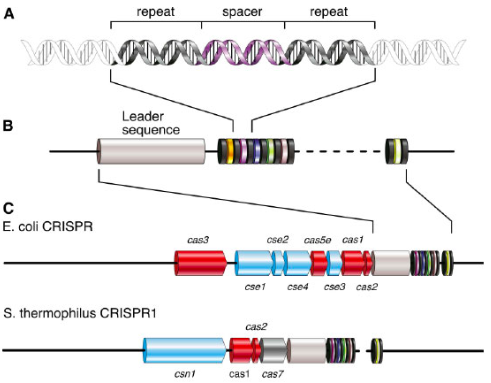
\includegraphics[scale=0.6]{crispr.png}
\caption{Structure du locus CRISPR-Cas, d'après\\ \url{https://www.sinobiological.com/crispr-locus.html}}
\end{figure}

Ces séquences incorporent dans les spacers des fragments d'ADN de bactériophages qui ont déjà infecté la bactérie qui sont stockés en vue de détecter et de détruire l'ADN de bactériophages similaires en cas d'infection ultérieure. Par conséquent, CRISPR-Cas est un système immunitaire naturel utilisé par les bactéries pour se protéger des infections virales. 

% Fonctionnement du système CRISPR-Cas 

\subsection{Fonctionnement du système CRISPR-Cas}

Les systèmes CRISPR-Cas sont de trois types et utilisent les différents gènes Cas pour intégrer des fragments de gènes étrangers dans les spacers de CRISPR. Par exemple, dans le cas d'une bactérie qui détecte la présence d'ADN ou d'ARN d'un virus, elle produit une enzyme nucléase appelée Cas9 capable de couper l'ADN viral, puis une séquence d'ARN CRISPR notée crARN correspondant à celle de l'ADN du virus et servant de guide ARN, puis finalement une séquence d'ARN traceur notée trARN. Lorsque trARN trouve sa cible parmi le génome du virus, Cas9 sectionne l'ADN viral puis en incorpore un fragment dans un espaceur du génome de la bactérie, conservant ainsi en mémoire une trace de ce virus en vue d'une éventuelle infection future. Les espaceurs servent donc de banque de mémoire en conservant l'ADN des virus qui ont attaqué la bactérie.

La technologie CRISPR-Cas9 s'inspire du système du même nom a d'abord été utilisée pour typer les souches bactériennes, suivant une technique appelée spoligotypage. CRISPR-Cas9 est actuellement principalement employé comme ciseau moléculaire afin d'éditer le génome et d'introduire localement des modifications génétiques.

% Spoligotyping

\section{Le spoligotypage}

La région DR du locus CRISPR-Cas présente un niveau de polymorphisme suffisant pour pouvoir classer phylogéographiquement les souches du MTBC. Le polymorphisme entre les différentes souches résulte des variations et de l'identité des spacers. C'est ce polymorphisme qui est exploité en 1997 par Kamerbeek et al. et expliqué dans \cite{kamerbeek} comme technique de génotypage spécifique du MTBC. Le \textit{Spacer Oligonucleotide Typing}, repose sur la détection de séquences répétitives trouvées entre les gènes d'un agent infectieux au sein d'un locus CRISPR-Cas. Pour ce faire, la région DR d'un isolat à tester subit un traitement par amplification PCR\footnote{\textbf{PCR Polymerase Chain Reaction} : méthode de réaction en chaîne utilisant un polymère pour dupliquer en grand nombre une séquence d'ADN spécifique. La méthode PCR repose sur le cycle thermique, qui expose les séquences à des cycles répétés de chauffage et de refroidissement pour permettre différentes réactions dépendantes de la température comme la fusion de l'ADN et la réplication de l'ADN par les enzymes. La méthode PCR utilise deux agents principaux : les polymères d'ADN i.e. des macromolécules répétant un même motif structural d'ADN et les amorces de séquençage.} ou celui d'une puce à ADN\footnote{\textbf{Puce à ADN} : ensemble de molécules d'ADN fixées sur une petite surface solide permettant de mesurer le niveau d'expression d'un grand nombre de gènes simultanément, ou de déterminer le génotype de plusieurs régions d'un génome.} pour dévoiler un motif de taches correspondant aux spacers. 

\begin{figure}[h!]
\centering
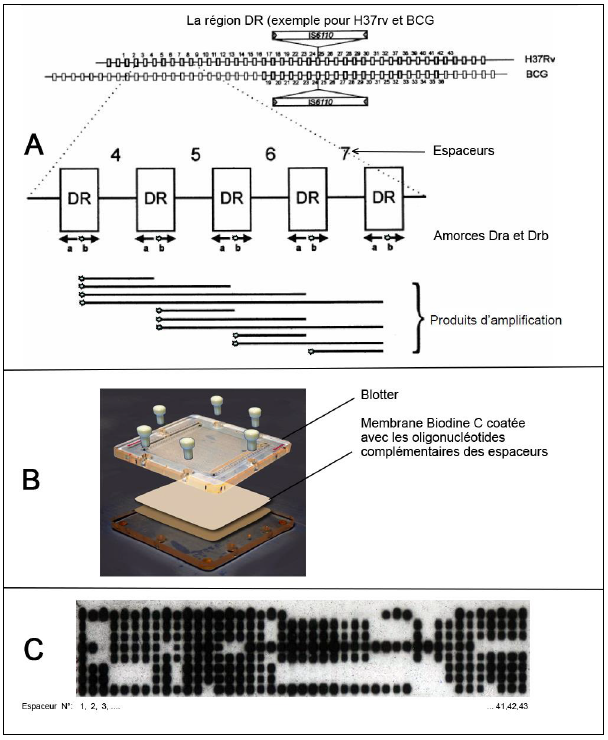
\includegraphics[scale=0.4]{spoligo.png}
\caption{Les différentes étapes du spoligotypage d'après \textit{Etudes descriptive, épidémiologique,\\ moléculaire et spatiale des souches Mycobacterium tuberculosis circulant à Antananarivo, Madagascar}}
\end{figure}

La comparaison de ces motifs permet la différentiation des souches. Quarante-trois espaceurs les plus polymorphes ont été utilisés pour le typage des mycobactéries suivant Kamerbeek et al. La classification classique de MTBC utilise donc un groupe de 43 bit représentant la présence ou l'absence d'espaceurs dans le locus CRISPR, qu'on appelle spoligotype. Des études pour augmenter le niveau de discrimination du spoligotypage ont été faites en 2010 utilisant 68 espaceurs. A l'heure actuelle l'équipe AND de l'université de Franche Comté utilise 98 espaceurs pour ce génotypage.

\begin{figure}[h!]
\centering
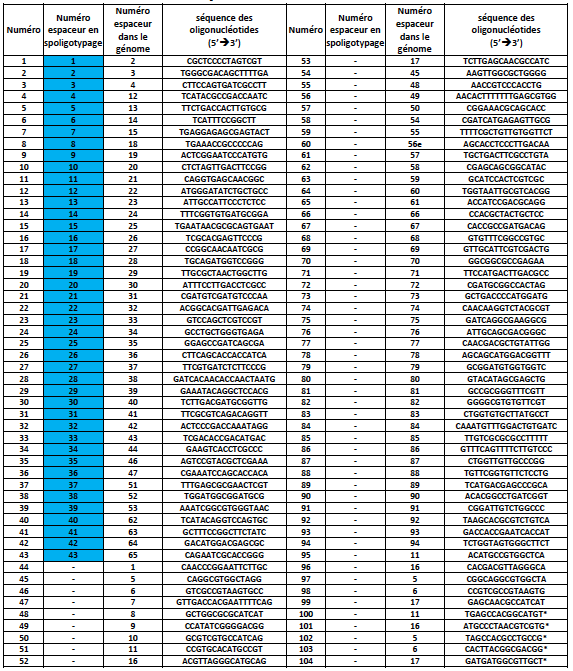
\includegraphics[scale=0.7]{spacer.png}
\caption{Espaceurs connus chez MBTC, d'après \textit{Etudes descriptive, épidémiologique, moléculaire\\ et spatiale des souches Mycobacterium tuberculosis circulant à Antananarivo, Madagascar}}
\end{figure}

La technique ne nécessite pas une importante quantité d'ADN car elle est basée sur une amplification de la région DR par PCR.
Les spoligotypes ainsi obtenus peuvent être partagées entre laboratoires et corroborent les résultats obtenus à partir d'autres marqueurs génétiques. Ces données numériques permettent de bien différencier les souches de tuberculosis et sont de moindre coût comparativement à d'autres méthodes. Cependant, le spoligotypage éprouve des difficultés à bien différencier les souches au sein de grandes familles de souches telles que la lignée 2 par exemple.

Le spoligotypage a permis de fournir une image globale de la diversité des souches de tuberculosis.

Une nouvelle technologie permettant de combiner le spoligotypage avec des tests moléculaires de sensibilité aux antituberculeux, appelée spoligoriftypage, a été développée pour aboutir à la version TB-SPRINT qui a été décrite en 2013 par Gomgnimbou et al. dans leur article \cite{gomgnimbou}. Elle consiste au typage tuberculose-spoligo-rifampicine-isoniazide fonctionnant sur des systèmes à base de microbilles, à partir notamment de 43 espaceurs, 11 SNPs présents sur rpoB aux positions 516, 526 et 531. Cette nouvelle génération de spoligotypage fournit donc, en plus des données classiques de génotypage, une prédiction basée sur la mutation des profils de résistance aux médicaments.

% Normalisation

\subsection{Vers une normalisation des spoligotypes}

Au début du spoligotypage, il n'existait pas de norme pour décrire les motifs formés par les spacers ou simplement les numéroter. Chaque laboratoire utilisait son propre système de numérotation accompagné d'un schéma descriptif du motif. Ce manque de normalisation entravait les possibilités de comparaison des résultats obtenus et le développement d'une vision mondiale de l'évolution de MTBC. Une méthode standardisée de description des spoligotypes a été proposée en 2001 par Dale JW dans son article \cite{dale}. 

Tout d'abord, une base de données centralisée regroupant tous les motifs connus et de leurs numérotations jusqu'à présent associées existe au RIVM Rijksinstituut voor Volksgezondheid en Milieuhygiene, Bilthoven, Netherlands. Elle peut être consultée au \url{http://www.caontb.rivm.nl}. A partir de 2001, les nouveaux motifs devraient prendre un unique format de numérotation pour être répertoriés dans cette base de données. Toutefois, cela nécessite l'interrogation systématique de la base de données et la comparaison avec les éléments déjà existants pour chaque nouveau spoligotype. Pour éviter cette perte de temps, de nombreux laboratoires utilisent des systèmes rationnels avec des codes descriptifs assignés à chaque isolat. 

Dale JW et al. dans leur article \cite{dale} proposent d'utiliser exclusivement un système rationnel octal ou hexadécimal, sachant qu'il est aisé de passer de l'un à l'autre et qu'il est également facile de retrouver l'état initial binaire. Ainsi, les motifs de spoligotype comprenant 43 bits seraient réduits dans le système octal en 14 groupes de 3 bits auquel s'ajouterait un unique bit, ce qui donnerait finalement un ensemble de 15 chiffres en écriture octale. En ce qui concerne le système hexadécimal, les motifs de 43 bits seraient réduits en 6 groupes de 8 bits avec un dernier groupe ne comprenant que 3 bits, soit 6 groupes de 2 chiffres hexadécimaux. Notons que un bit symbolise dans ce cas la présence ou l'absence d'une espaceur dans le locus étudié.

\begin{figure}[h!]
\centering
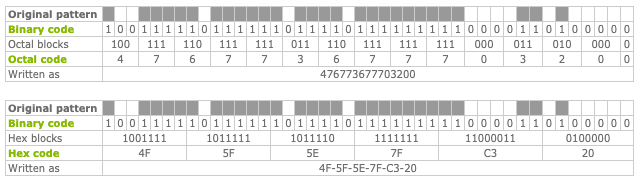
\includegraphics[scale=0.6]{hexa.png}
\caption{Exemple de système rationnel octal et hexadécimal, d'après\\ \url{https://www.mbovis.org/spoligotype-nomenclature.php}}
\end{figure}

Le site Mbovis.org, \url{https://www.mbovis.org/database.php}, bien que dédié aux souches animale de MTBC, fournit une application pratique permettant de transformer rapidement les spoligotypes binaires en système octal ou hexadéciamal.

% Spolpred et SpoTyping

\subsection{Quel outil informatique pour le spoligotypage ?}

Les technologies PCR de génotypage utilisent toujours différents marqueurs tels que les SNPs pour obtenir en laboratoire des résultats fiables. Des logiciels informatique de prédiction du génotype ont également fait leur apparition pour optimiser les coûts et le gain de temps. Ils offrent un outil de comparaison des résultats obtenus expérimentalement et in silico.

SpolPred est un logiciel de prédiction rapide et précis des spoligotypes de tuberculosis à partir de séquences génomiques courtes appelées reads\footnote{\textbf{Read} : mélange de courtes séquences oligonocléotidiques de 20 à 200 pb généré par des séquenceurs}. Cet outil développé par Preston M. fonctionne efficacement avec des reads provenant de plateformes telles que Illumina GAII ou HiSeq. SpolPred utilise des fichiers de séquences de reads simples ou par paires au format FASTQ, pour produire une prédiction de spoligotype au format octal qui est comparée au spoligotype correspondant dans la base SITVIT.

\begin{figure}[h!]
\centering
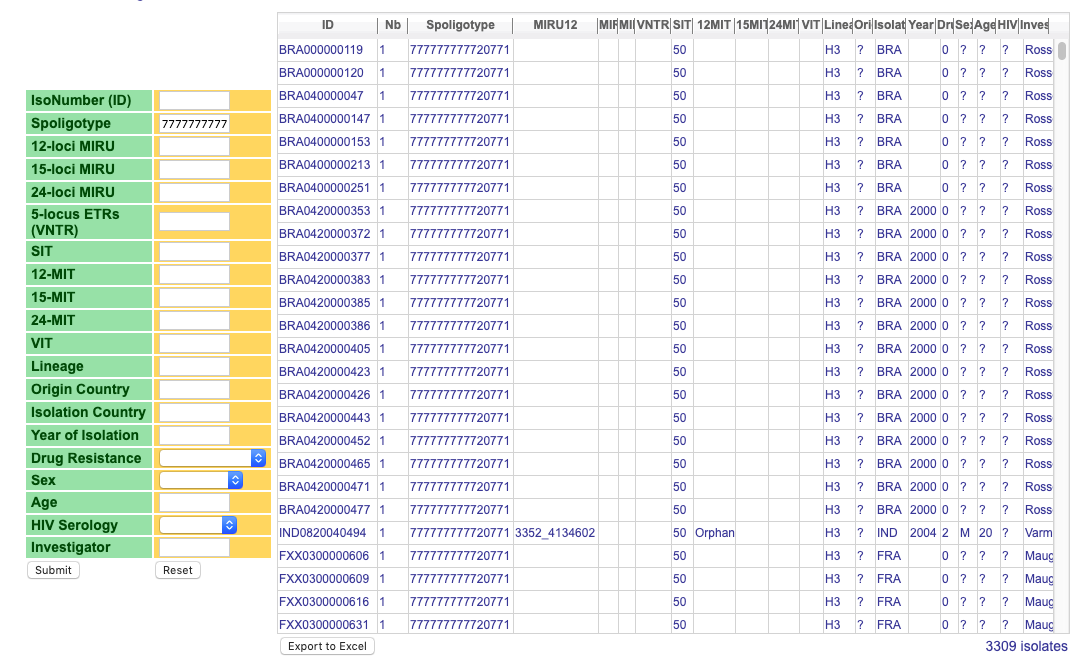
\includegraphics[scale=0.44]{spol.png}
\caption{Exemple de recherche effectuée sur SITVIT2 à partir du spoligotype 777777777720771 dont le résultat est exploitable au format Excel}
\end{figure}

Dans leur étude, Coll F. et al.\cite{coll} montrent en 2012 l'utilité de SpolPred en comparant les spoligotypes obtenus par le logiciel avec les résultats de laboratoire. Ils dévoilent ainsi les limites de la méthode expérimentale qui a répertorié cinq faux spoligotypes, alors que SpolPred a su éviter une erreur de classification du génotype. Par ailleurs, il apparaît que SpolPred offre plus de rapidité et des résultats pratiquement identiques à ceux obtenus avec la méthode bioinformatique par assemblage, consistant à fusionner des fragments d'ADN issus d'une plus longue séquence afin de reconstruire la séquence originale, à l'aide du logiciel Velvet développé en 2008.

Toutefois, d'après l'étude de Xia et al.\cite{xia}, la précision de SpolPred est fortement réduite lorsque les reads n'ont pas une taille uniforme, comme par exemple lorsqu'ils proviennent de séquençages Ion Torrent ou de la plateforme de diagnostique clinique Illumina MiSeq. Ainsi, lorsque les reads ne sont pas uniformes, la précision des résultats dépend fortement de leurs tailles et donc du choix initial fait par l'opérateur. Par ailleurs, SpolPred demande à l'utilisateur de spécifier la direction de lecture des reads, et le logiciel n'utilise donc qu'une partie des informations fournies par les reads.

Une problématique de SpolPred en 2020 est que le logiciel n'est plus disponible au public. En effet, une visite sur le site officiel \url{http://www.pathogenseq.org/spolpred} fourni comme référence dans le document \cite{coll} de Coll F. et al. montre que le nom de domaine est à vendre. Preston M., qui a fait partie de l'équipe de rechercher de Coll F. pour le développement de SpolPred, a bien créé un site \url{https://www.mybiosoftware.com/spolpred-predict-the-spoligotype-from-raw-sequence-reads.html} proposant le téléchargement du logiciel, mais le lien est actuellement inactif.

Une alternative à SpolPred est SpoTyping présenté en 2016 dans l'article \cite{xia} de Xia et al. comme étant 20 à 40 fois plus rapide que SpolPred pour prédire avec précision des spoligotypes de tuberculosis à partir de reads de taille uniforme ou variable. Par ailleurs, SpoTyping lit chaque read dans les deux directions en exploitant complètement les informations fournies. SpoTyping réduit la durée des recherches en intégrant l'algorithme BLAST\footnote{\textbf{BLAST Basic Local Alignment Search Tool} : logiciel basé sur l'algorithme du même nom qui détecte des régions similaires entre plusieurs séquences biologiques. Le programme compare les séquences de nucléotides aux séquences contenues dans la base de données BLAST pour fournir des résultats statistiquement significatifs.} dans ses calculs. Il compare les isolats testés avec ceux ayant le même spoligotype dans la base de données mondiale SITVIT, qui regroupe les données épidémiologiques\footnote{\textbf{Epidémiologie} : discipline scientifique qui étudie les problèmes de santé dans les populations humaines, leur fréquence, leur géographie ainsi que les facteurs influants.} associées à des isolats de même spoligotype.

SpoTyping utilise des fichiers de séquences de reads simples ou par paires au format FASTQ et des fichiers de séquences complètes de génomes ou de contigs assemblés au format FASTA. Le séquences de reads sont regroupés en une unique séquence continue au format FASTA pour être ensuite soumis à l'algorithme BLAST qui détecte les régions similaires. Finalement la base de données SITVIT permet d'identifier les isolats ayant le même spoligotype. SpoTyping est limité à une lecture de 250 Mbp au sein des séquences de reads testées, lors de l'utilisation du swift mode qui accélère le temps de traitement.

SpoTyping propose un rapport statistique permettant de résumer le rapprochement avec les spoligotypes trouvés dans la base de données SITVIT, ainsi qu'une estimation du nombre de correspondances positives pour chaque spacer.

L'étude de Iwai H. et al. \cite{iwai} montre l'intérêt d'une analyse de MTBC à l'aide de serveurs, appelée CASTB, et notamment le spoligotypage. Le Webserver fournit une vue complète des données, mais les performances de chaque outil utilisé ne sont pas décrites dans l'article. Il est probable que le spoligotypage prenne plus de temps en passant par un serveur suite au problème de disponibilité des données et aux lenteurs de téléchargement de ces données. Il semblerait que SpoTyping, de par sa configuration locale, puisse fournir un résultat en une minute.

\begin{figure}[h!]
\centering
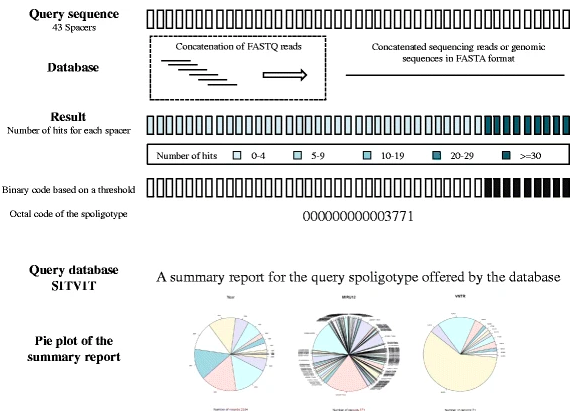
\includegraphics[scale=0.6]{spotyping.png}
\caption{Exemple de fonctionnement de SpoTyping, d'après \textit{SpoTyping:\\ fast and accurate in silico Mycobacterium spoligotyping from sequence reads}}
\end{figure}

D'après le repository \url{https://github.com/xiaeryu/SpoTyping-v2.0/blob/master/SpoTyping-v2.0-commandLine/SpoTyping-README.pdf}, les spécifications techniques sont les suivantes :

SpoTyping peut s'exécuter sur les principaux systèmes d'exploitation, contrairement à SpolPred qui utilise exclusivement Linux. Il se présente à la fois sous forme de script et sous forme d'application avec une interface graphique.

SpoTyping est un logiciel open-source qui peut se télécharger gratuitement à l'adresse \url{https://github.com/xiaeryu/SpoTyping-v2.0}. SpoTyping nécessite l'utilisation de Python2.7 et BLAST.

Le fichier obtenu propose une prédiction de spoligotype au format de code binaire et octal. Le fichier log obtenu contient de nombre de correspondances positives des résultats de BLAST pour chaque séquence de spacer. Le fichier xls Excel obtenu fournit le resultat de la recherche de spoligotype auprès de la base de données SITVIT2\footnote{\textbf{Base de données SITVIT2} : mise à jour de la base de données SITVIT, consultable en ligne \url{http://www.pasteur-guadeloupe.fr:8081/SITVIT2/index.jsp}}.

Il est recommandé d'utiliser le swift mode paramétré par défaut si le débit de séquençage\footnote{\textbf{Séquençage du génome} : consiste, par des méthodes chimiques ou de biologie moléculaire, à déterminer l'ordre des nucléotides de l'ADN.} est inférieur à 135 Mbp. Pour les débits de séquençage inférieurs à 135 Mbp ou supérieurs à 1260 Mbp, les seuils doivent être réglés entre 0.018 et 0.1486 fois la profondeur de lecture estimée pour les hits sans erreur, et entre 0.018 et 0.1488 fois la profondeur de lecture estimée pour les hits tolérant une erreur. Notons que la profondeur de lecture est définie par le débit de séquençage divisé par 4 500 0000 qui correspond à l'estimation de la longueur d'un génome de MTBC.

\subsection{Comparaison de spoligotypes}

Une fois les spoligotypes de différentes lignées obtenus, il est nécessaire de les comparer pour chercher à faire ressortir les points communs ou certains traits pouvant être liés à une muttion particulière. Il existe à l'heure actuelle un premier outil en ligne de comparaison du nom de SpolSimilaritySearch, accessible à l'adresse \url{http://www.pasteur-guadeloupe.fr:8081/SpolSimilaritySearch/index.jsp}, et présenté par Couvin D. et al. \cite{couvin}, utilisant la base de données SIVIT2 pour rechercher des similitudes entre spoligotypes.

Cet outil pourrait donc s'avérer utile pour commencer à chercher des liens entre les sept lignées de \textit{M. tuberculosis} et les spoligotypes de différentes souches.

\begin{figure}[h!]
\centering
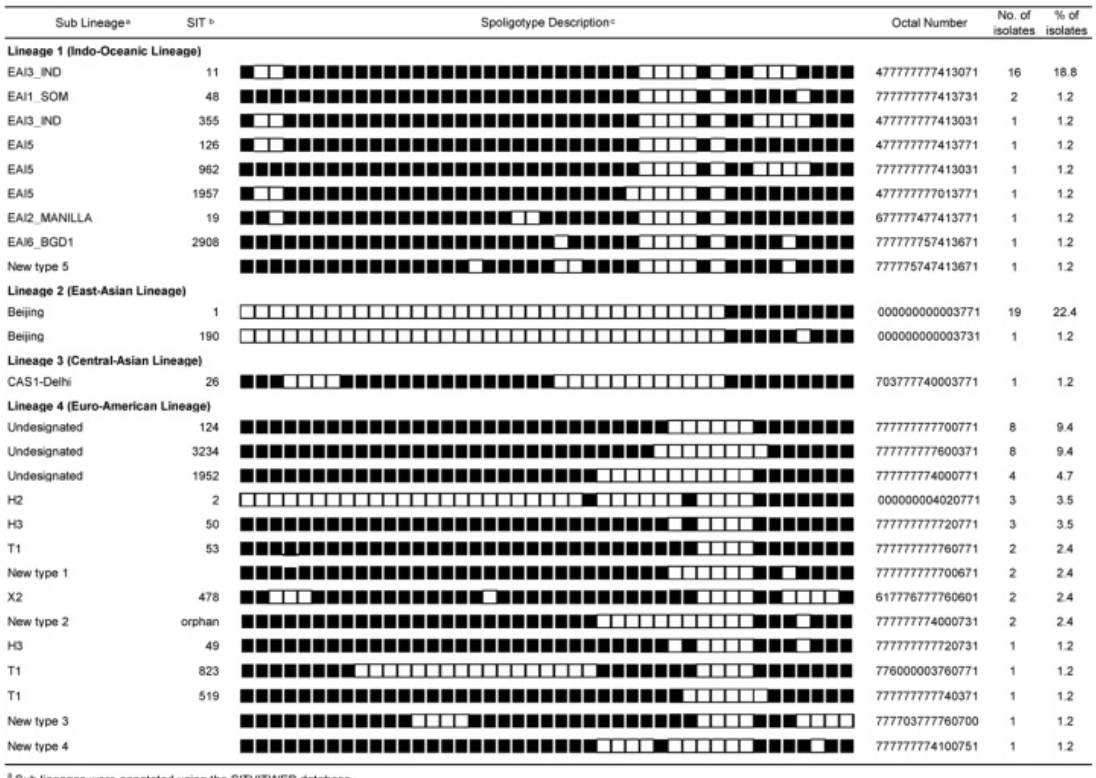
\includegraphics[scale=0.4]{comparaison.png}
\caption{Exemple comparatif de 26 spoligotypes correspondant à 4 lignées différentes de \textit{M. tuberculosis}, d'après \textit{Insight into genetic diversity of Mycobacterium tuberculosis in Kandy, Sri Lanka reveals predominance of the Euro-American lineage}}
\end{figure}

Par exemple, dans le tableau ci-dessus, si on sélectionne le spoligotype 777777777720771 appartenant à la lignée H3, et qu'on interroge la base SpolSimilaritySearch, on obtient les rapprochements suivants :

\begin{figure}[h!]
\centering
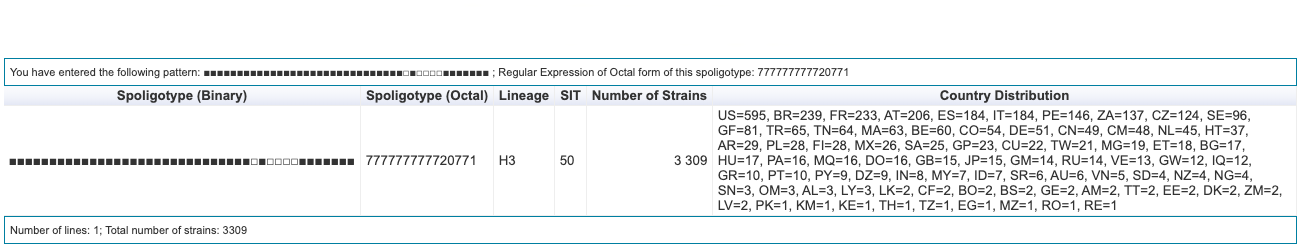
\includegraphics[scale=0.37]{spolsimilarity.png}
\caption{Recherche effectuée sur le site SpolSimilaritySearch}
\end{figure}

%the MRCA of extant M. tuberculosis seems to have existed as recently as 4,000-6,000 years ago
% finir lecture arcticle 3

% =========
% BIBLIOTHEQUE
% =========
\begin{spacing}{0.5}
\bibliographystyle{}
\renewcommand{\bibname}{Références}
\begin{thebibliography}{10}
\bibitem{comas}Comas I. et al. \textit{Out-of-Africa migration and Neolithic coexpansion of Mycobacterium tuberculosis with modern humans}, Nat Genet. 45(10): 1176–1182. doi:10.1038/ng.2744\\ \\

\bibitem{coll}Coll F. et al., \textit{SpolPred : rapid and accurate prediction of Mycobacterium tuberculosis spoligotypes from short genomic sequences}, Bioinformatics. 28(22):2991–3\\ \\

\bibitem{brynildsrud}Brynildsrud O.B. et al., \textit{Global expansion of Mycobacterium tuberculosis lineage 4 shaped by colonial migration and local adaptation}, 4(10): eaat5869. doi: 10.1126/sciadv.aat5869\\ \\

\bibitem{driscoll}Driscoll J. R., \textit{Spoligotyping for molecular epidemiology of the Mycobacterium tuberculosis complex}, 551:117-28. doi: 10.1007/978-1-60327-999-4 10\\ \\

\bibitem{jinek}Jinek M. et al, \textit{A programmable dual-RNA-guided DNA endonuclease in adaptive bacterial immunity}, 337(6096):816-21. doi: 10.1126/science.1225829\\ \\

\bibitem{gori}Gori A. et al, \textit{Spoligotyping and Mycobacterium tuberculosis}, 11(8): 1242–1248. doi: 10.3201/1108.040982\\ \\

\bibitem{perry1}Perry S. et al., \textit{Infection with Helicobacter pylori is associated with protection against tuberculosis}, 5(1):e8804. doi: 10.1371/journal.pone.0008804\\ \\

\bibitem{perry2}Perry S. et al, \textit{The immune response to tuberculosis infection in the setting of Helicobacter pylori and helminth infections}, 141(6): 1232–1243. doi: 10.1017/S0950268812001823\\ \\

\bibitem{xia}Xia E. et al., \textit{SpoTyping: fast and accurate in silico Mycobacterium spoligotyping from sequence reads}, 8:19. doi 10.1186/s13073-016-0270-7\\ \\ 

\bibitem{dale}Dale JW. et al., \textit{Spacer oligonucleotide typing of bacteria of the Mycobacterium tuberculosis complex: recommendations for standardised nomenclature.}, 5(3):216–9\\ \\

\bibitem{iwai}Iwai H et al., \textit{CASTB (the comprehensive analysis server for the Mycobacterium tuberculosis complex): A publicly accessible web server for epidemiological analyses, drug-resistance prediction and phylogenetic comparison of clinical isolates. Tuberculosis.}, 95(6):843–4\\ \\

\bibitem{demay}Demay C. et al., \textit{SITVITWEB - A publicly available international multimarker database for studying Mycobacterium tuberculosis genetic diversity and molecular epidemiology.}, Infect Genet Evol. 12:755–66\\ \\

\bibitem{}McGovern Institute Channel, \textit{Genome Editing with CRISPR-Cas9}, \url{https://www.youtube.com/watch?v=2pp17E4E-O8}\\ \\

\bibitem{oneil}O'Neil M.B. et al., \textit{Lineage specific histories of Mycobacterium tuberculosis dispersal in Africa and Eurasia}, bioRxiv. 10.1101/210161\\ \\

\bibitem{ratovonirina}Ratovonirina N. H., \textit{Etudes descriptive, épidémiologique, moléculaire et spatiale des souches Mycobacterium tuberculosis circulant à Antananarivo, Madagascar}, Thèse de Doctorat de l'Université Paris-Saclay\\ \\

\bibitem{kamerbeek}Kamerbeek et al., \textit{Simultaneous detection and strain differentiation of Mycobacterium tuberculosis for diagnosis and epidemiology}, 35(4): 907–914\\ \\

\bibitem{mendis}Mendis C. et al., \textit{Insight into genetic diversity of Mycobacterium tuberculosis in Kandy, Sri Lanka reveals predominance of the Euro-American lineage}, International Journal of Infectious Diseases 87 84-91\\ \\

\bibitem{gomgnimbou},Gomgnimbou M. K. et al., \textit{Tuberculosis-Spoligo-Rifampin-Isoniazid Typing: an All-in-One Assay Technique for Surveillance and Control of Multidrug-Resistant Tuberculosis on Luminex Devices}, 51(11):3527-34. doi: 10.1128/JCM.01523-13\\ \\

\bibitem{couvin}Couvin D. et al., \textit{SpolSimilaritySearch - A web tool to compare and search similarities between spoligotypes of Mycobacterium tuberculosis complex}, 105:49-52. doi: 10.1016/j.tube.2017.04.007

\end{thebibliography}
\end{spacing}
\end{document}